\documentclass[text.tex]{subfiles}

\begin{document}


\section{8-fold rotational symmetry}
\subsection{Definition}
\begin{align*}
x^2 &=2x+1 &
\beta_8 &= 1 + \sqrt{2} \doteq 2.414 &
\beta_8' &= 1 - \sqrt{2} \doteq -0.414 \\
\end{align*}

\subsection{Formulas}
\begin{align*}
\beta_8\beta_8' &= -1 &
\beta_8 + \beta_8' &= 2 &
\beta_8^{k+2} &= 2\beta_8^{k+1} + \beta_8^k \\
\end{align*}

\subsection{Distances}
\begin{remark}
$\frac{1}{\beta_8} = \beta_8-2$
\end{remark}
\begin{table}[h!]
\begin{center}
\begin{tabular}{c|ccccc}
	\toprule
		\begin{tabular}[x]{@{}c@{}}Window\\size\end{tabular}&$\beta_8-2$	&	$\left( \beta_8-2, 3-\beta_8 \right)$	&	$3-\beta_8$	&	$\left( 3-\beta_8, \beta_8 \right)$	&	$\beta_8$	\\
	\midrule
		&$3\beta_8+1$ 	&	$3\beta_8+1$	&				&				&				 	\\ 
		&$2\beta_8+1$	  &	$2\beta_8+1$	&	$2\beta_8+1$	&	$2\beta_8+1$	&				\\
		Distances&			&	            	&	            	&	$\beta_8+1$	&	$\beta_8+1$			\\
		&			          &	$\beta_8$		  &	$\beta_8$		  &	$\beta_8$		&	$\beta_8$		\\
	\bottomrule
\end{tabular}
%\caption{All possible distances between two consecutive points of the sequence of the quasicrystal with a window of the given size.}
\label{table:spaces}
\end{center}
\end{table}

\subsection{List of Voronoi tiles}
$\beta_8-2$
$\left( \beta_8-2, 3-\beta_8 \right)$
$3-\beta_8$
$\left( 3-\beta_8, \beta_8 \right)$
$\beta_8$	

\begin{figure}[h!]
\centering
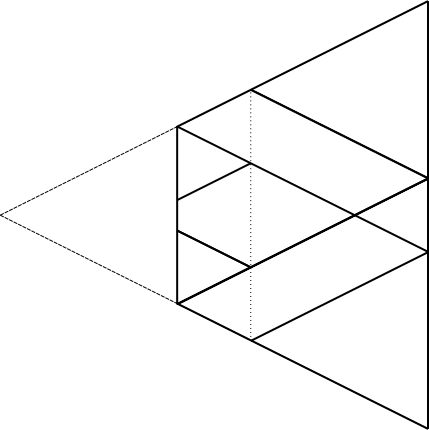
\includegraphics[width=0.74\textwidth]{img/1D/alpha}
\caption{Division of window into sections corresponding to different Voronoi tiles. Each vertical slice of the trapezoid represents a single window of size in $[\beta_8-2,1]$. The diagonal lines divide each window into the sections corresponding to different Voronoi tiles. }
\label{fig_8fold1DWindow}
\end{figure}

\end{document}
